% Template for PLoS
% Version 1.0 January 2009
%
% To compile to pdf, run:
% latex plos.template
% bibtex plos.template
% latex plos.template
% latex plos.template
% dvipdf plos.template

\documentclass[12pt]{article}

% amsmath package, useful for mathematical formulas
\usepackage{amsmath}
% amssymb package, useful for mathematical symbols
\usepackage{amssymb}

% graphicx package, useful for including eps and pdf graphics
% include graphics with the command \includegraphics
\usepackage{graphicx}
\usepackage{epstopdf}

% cite package, to clean up citations in the main text. Do not remove.
\usepackage{cite}

\usepackage{color} 

% Use doublespacing - comment out for single spacing
\usepackage{setspace} 
\doublespacing


% Text layout
\topmargin 0.0cm
\oddsidemargin 0.5cm
\evensidemargin 0.5cm
\textwidth 16cm 
\textheight 21cm

% Bold the 'Figure #' in the caption and separate it with a period
% Captions will be left justified
\usepackage[labelfont=bf,labelsep=period,justification=raggedright]{caption}

% Use the PLoS provided bibtex style
\bibliographystyle{plos2009}

% Remove brackets from numbering in List of References
\makeatletter
\renewcommand{\@biblabel}[1]{\quad#1.}
\makeatother


% Leave date blank
\date{}

\pagestyle{myheadings}
%% ** EDIT HERE **


%% ** EDIT HERE **
%% PLEASE INCLUDE ALL MACROS BELOW

%% END MACROS SECTION

\begin{document}

% Title must be 150 characters or less
\begin{flushleft}
{\Large
\textbf{Computational Identification and Annotation of Key-reactions in Metabolic Pathways of E. coli that Discriminate Different Growth Conditions.}
}
\bigskip
\noindent
% Insert Author names, affiliations and corresponding author email.
\\
Viswanadham Sridhara$^{1}$,
Austin G. Meyer, 
Jeffrey E. Barrick$^{1,2}$,
Pradeep Ravikumar$^{3}$,
Daniel Segre$^{4}$, 
Claus O. Wilke$^{1,5,\ast}$
\\
\bigskip
\bf{1} Center for Computational Biology and Bioinformatics, The University of Texas at Austin, Austin, TX, USA
\\
%\\[3\baselineskip]
\bf{2} Department of Chemistry and Biochemistry, The University of Texas at Austin, Austin, TX, USA
\\
%\\[3ex]
\bf{3} Department of Computer Science, The University of Texas at Austin, Austin, TX, USA
\\
%\\[3ex]
\bf{4} Department of Biology, Boston University, Boston, MA, USA
\\
%\\[3ex]
\bf{5} Section of Integrative Biology, The University of Texas at Austin, Austin, TX, USA
\\
%\\[3ex]
\bigskip
$\ast$ E-mail: wilke@austin.utexas.edu
\end{flushleft}
%\\
% Please keep the abstract between 250 and 300 words
\newpage
\section*{Abstract}
Biochemical information about the enzymes catalyzing reactions in metabolic pathways of microbes is obtained from databases, such as BiGG, BioCyc. This information along with flux balance analysis (FBA) is routinely used in metabolic engineering applications. Here, we generated metabolic flux data using FBA in E. coli for different growth conditions. We then used model selection algorithm, LASSO, for identifying the key reactions that discriminate different growth conditions. In this study, we used 7 each of carbon/nitrogen sources along with more commonly used experimental media to grow K-12 MG1655 strain. We showed that separately predicting the carbon and nitrogen sources in carbon-nitrogen mixture is better than jointly predicting. These models on average predict 9 features per growth conditions for carbon/nitrogen sources. The misclassification rate seems to increase with increasing background noise levels and decreasing training data size. We then mapped these features (reactions) on the E. coli central carbon metabolism to visually show the key genes/metabolites specific to a particular growth condition. For the more commonly used growth media, the models seems to predict at high accuracy too. 

% Please keep the Author Summary between 150 and 200 words
% Use first person. PLoS ONE authors please skip this step. 
% Author Summary not valid for PLoS ONE submissions.   

\section*{Author Summary}
Predicting the biomass composition, co-factors yield using FBA techniques on computational metabolic models is gaining popularity in the last decade. Moreover, metabolic pathways provide us a framework to integrate diverse kinds of high-throughput data i.e., transcriptomics/proteomics/metabolomics data. Here, we generated metabolic fluxes for different growth conditions and then used machine learning techniques to predict the key-reactions that discriminate different growth conditions. Such automatic identification of key-reactions would in turn also help experimentalists to quantitatively measure the respective metabolites involved (mass-spec based metabolomics), proteins that catalyze the reactions (mass-spec based proteomics) or the genes that encode these enzymes (sequencing based RNA-seq experiments).

\section*{Introduction}
Flux balance analysis (FBA) is a technique used routinely for computational guidance in metabolic engineering experiments \cite{Orthetal2010}. FBA requires a metabolic model, which generally is obtained from genome sequence and its annotations. The metabolic models of few species are well developed over the past decades, given the advances in genome sequencing \cite{Schellenbergeretal2010,Caspietal2012}. Determining enzyme kinetics for metabolic reactions is extremely difficult and hence constrained based methods like FBA that calculate steady-state flux vector have gained importance.

\bigskip
\noindent
The genome sequence, its annotation along with the massive amounts of biochemical data available from the literature are the key ingredients for metabolic reconstructions \cite{EdwardsPalsson2000, Karpetal1996, OuzounisKarp2000}. Among prokaryotes, E. coli metabolic model has been very well annotated  by several groups \cite{Karpetal1996,EdwardsPalsson2000}. Palsson's group has been extensively updating the E. coli metabolic model over the last 2 decades \cite{EdwardsPalsson2000,Reedetal2003,Feistetal2007,Orthetal2012}. Similarly Karp's group at SRI is updating their model for more than 2 decades and stored the content as EcoCyc pathway genome database \cite{Keseleretal2013}. 

\bigskip
\noindent
At the same time, the experimental data can be used to refine the constraints used in these flux balance analysis. Recently, gene expression profile data is used to refine the bounds of reaction fluxes in metabolic models, which in turn helped improve prediction of input carbon sources \cite{Brandesetal2012}. There is still lot of room for improvement, given the different kinds of possible constraints \cite{Priceetal2004}.

\bigskip
\noindent
There was a study that identified minimal set of reactions that are necessary for growth for a particular growth condition \cite{Burgardetal2001}. Likewise, there was another study published recently that identified minimal set of nutrients for growth conditions \cite{Ekeretal2013}. Another study by Ibarra et. al., \cite{Ibarraetal2002} looked at the growth of E. coli K-12 MG1655 strain on glycerol for 40 days (~700 generations) and they saw an increase in the growth rate with generations. These are some of the studies that indicate diverse applications of metabolic engineering that use FBA.
 
\bigskip
\noindent
The metabolic pathways, apart from providing a genotype-phenotype relationship, also provide a good resource to integrate diverse kinds of data, such as DNA sequence, mass-spectrometry data. For example, combining flux analysis data with phosphoproteomics data to deduce functionality of enzymes is described in this study \cite{Oliveiraetal2012}. An interesting study to understand the adaptation of yeast metabolism to the growth conditions is studied, using enzymes in metabolic model pathways to validate the quantitative proteomics data \cite{Costenobleetal2011}. Other than the above studies, this set of pathways when integrated with other diverse types of data, have many applications as discussed in these 2 reviews \cite{Hydukeetal2013,Oberhardtetal2009}.

\bigskip
\noindent
As shown by \cite{Almaasetal2004}, for a particular design (growth type/mutant etc) there are many reactions that have low reaction flux, but the ones with high-flux typically provide information on the growth condition or the mutant type. To our knowledge, there were no studies that identified growth sources from flux data. Here, we used machine learning techniques to predict these sources from patterns of simulated flux data.

\bigskip
\noindent
Machine learning algorithms use with computational biology has been growing. In biological data, generally the number of samples is far less than features. So, linear models cannot be used without reducing the number of covariates.  For example, differential expression of tens of thousands of genes in microarray studies or identifying the SNPs in GWAS studies is a routine task in biomedical research now-a-days. Even though the sequencing technologies are becoming cheaper day-by-day, the number of samples sequenced is still low, compared to the number of features. In such cases, model selection algorithm LASSO \cite{Tibshirani1996} seems to perform well. LASSO methods are used in the past for genomics studies \cite{Wuetal2009}. LASSO seems to perform well with other kinds of data, for example, classifying structural images of brain using MRI data \cite{Casanovaetal2011,Casanovaetal2012,Wangetal2012}.

\bigskip
\noindent
There are many R and MATLAB packages that can be used for LASSO. GLMNET  \cite{Friedmanetal2010} is one such package that can be used for methods based on convex penalties (lasso, ridge-regression, elastic net etc). This package also comes with algorithmic efficiency and speed \cite{Friedmanetal2010}. GLMNET is shown to work on large datasets and with many labels. Given the sparsity of the reaction flux data, we used GLMNET \cite{Friedmanetal2010} for classifying different growth conditions.

% Results and Discussion can be combined.
\section*{Results}

Improving the growth rate or identifying the enzymes key for improving specific metabolite concentrations is a routine task in metabolic engineering. FBA can be regarded as a technique to computationally guide experimentalists, for example, picking a specific mutant or growth condition that increases a particular engineering target of interest. Here, we used FBA with machine learning techniques to predict growth sources from simulated flux data.

\bigskip
\noindent
1. For FBA, we used COBRA toolbox \cite{Schellenbergeretal2011} with MATLAB.

\bigskip
\noindent
2. For classification, we used GLMNET \cite{Friedmanetal2010} package with R.

\bigskip
\noindent
3. We used E. coli model iAF1260, downloaded from BiGG database \cite{Schellenbergeretal2010}.

\noindent
Below we describe the results obtained in this study.

\subsection*{Simulating metabolic flux datasets:}
The iAF1260 metabolic model of K-12 MG1655 strain was obtained from BiGG database \cite{Schellenbergeretal2010}. This model has 2382 reactions, that included the transport, biochemical and biomass composition reaction. In this model, we removed all the transport reactions as these are collinear to the input growth sources, which we are trying to predict from flux data. Other details about this model are provided in methods section.

\bigskip
\noindent
For different input growth conditions that are listed in Table 1, we generated fluxes. To see the effect of noise, we added randomly picked carbon and nitrogen sources that were previously used \cite{Feistetal2007}. Use of noise also allows us to generate many replicates for the same combination of sources, although other ways of finding alternate optima exists \cite{MahadevanSchilling2003}.

\bigskip
\noindent
We generated 100 replicates of pairwise combinations of 7 carbon and 7 nitrogen sources, i.e., 4900 observations. We then divided the dataset into training and test sets. We trained the models with training data using GLMNET package and used the test set for calculating the misclassification rates. We generated flux data and calculated misclassification rates in the same manner for other commonly used media described in Table 2. Below, we summarize the results.

\bigskip
\subsection*{Noise and training data size effects}
Keeping the uptake rate at 1\% (0.2 mmol/gDWhr) of the primary sources, we changed the number of background sources that we used as noise. For example, 2\% noise means that we randomly picked 2 carbon and 2 nitrogen sources from a set of 174 carbon and 78 nitrogen sources used previously \cite{Feistetal2007}. We used the cross-validation GLMNET to pick the model (regression coefficients). We did this for varying noise levels and training data size.

\bigskip
\noindent
Figure 2 shows that as background carbon and nitrogen sources interference increases, the misclassification rate increases. This is the case for both jointly predicting and separately predicting carbon and nitrogen sources. At 1\% noise, the difference between joint and separate predictions is not a lot, but clearly at 10\% noise, misclassification rate is lower for separate prediction. This result has 2-fold advantages. 1. The classification models can be built by traning individual sources, making the classification relatively easy. 2. Since the number of experimental observations are generally small, joint prediction has less data to train compared to individual prediction. Even at 10\% noise level with joint prediction, the misclassification rate is 25\% using these models. On the other hand, given 7 carbon and 7 nitrogen sources, just by chance the misclassification rate is expected at 93\%.

\bigskip
\noindent
Most of the carbon sources uptake seems to be limited by nitrogen and few nitrogen sources seems to have limited carbon for their growth. So, we changed the uptake rates of carbon and nitrogen sources so that there is no limiting factor and re-analyzed by training a new model. There seems to be no effect of these uptake rates, hence validating the above model's accuracy.

\bigskip
\noindent
Figure 3 shows the effect of training data size on misclassification rate.  Clearly, with a large training data set size of ~2400 observations, the classification is better compared to that of ~480 observations.

\bigskip
\noindent
Figure 4 is a heatmap for C/N predictions at different noise levels. The results indicate that as noise level increases from 1\% to 20\%, carbon sources get predicted as actate, while N sources get predicted as ammonia. Looking at the reactions that are predicted by GLMNET for acetate and ammonia sources, it seems that they either are part of the TCA cycle or lead to the TCA cycle. This might be due to the objective function used, which is maximizing biomass composition. Generally with any input growth source, the reactions in the pathway that lead to TCA should have some reasonable amount of flux calculated by FBA, if the key is to produce biomass.

\bigskip
\noindent
The number of predictors for a particular source on the average is ~9. This is relatively small given the total number of 1443 reactions. To test the accuracy of the models, we used a simpler strategy. For each reaction that has a non-zero weight in the model, we knocked-off that reaction, trained a new model (separate prediction) and calculated the test accuracy. Except for 3 reactions (predictors), the misclassification rate with the newer models seems to be the same for the rest 126 key-reactions (features predicted for 7 carbon and 7 nitrogen sources). This indicates the accuracy of the model and also indicate that alternate models exist for unique set of reactions.

\bigskip
\noindent
As a further test, we obtained simulated flux measurements using maltose as carbon source and the 7 nitrogen sources used earlier. Individual prediction seems to classify maltose as glucose more than 85% of the times. The nitrogen sources were predicted correctly more than 95% of the times. However, when we tried to predict using the joint model, the nitrogen sources were mispredicted most of the times. The carbon source 'maltose' was predicted as D-sorbitol most of the times. On the other hand, most of the nitrogen sources were predicted as putrescine. 

\subsection*{Mechanistic Insights}

\bigskip
\noindent
To have mechanical insights into the predicted reactions, we mapped these reactions onto the E. coli central metabolism model. We overlayed these reactions on E. coli central metabolism along with the metabolites that are both consumed and produced by the reaction. Manual validation of these reactions indicate that indeed some reactions seem specific to growth source, for example "XXXX" reaction specific to "YYYY" source \cite{ZZZZ}. E. coli metabolic map showing predicted reactions for 4 carbon and nitrogen sources is shown in figures 4 and 5. All reactions that are predicted by GLMNET is provided in supplementary information 1.

\bigskip
\subsection*{Large-scale prediction of Carbon/Nitrogen sources}
Since individual prediction is shown to perform better than joint prediction, we did large-scale prediction of the comprehensive list of 174 carbon and 78 nitrogen sources. We used the similar methodology as we used earlier i.e., we generated simulated fluxes for all pair-wise combinations of carbon/nitrogen sources (174*78) for 2 replicates. We used 1 replicate for training the model and then we used the 2nd replicate for testing. The misclassification rate for carbon sources is X\%, while the misclassification rate for nitrogen sources is Y\%.  

\bigskip
\subsection*{Further validation with other media}
We did similar analysis for the media that are more commonly used in E. coli experiments. The media we used were AB minimal media, ATCC media, Davis Mingioli media and Bochneder defined minimal media. Since the number of different media used in our analysis was 4, we were able to classify at a higher rate even at higher noise levels and lower number of replicates. The misclassification rate with the test set is found to be less than 1\% for noise levels upto 20\%. There was only one feature predicted for each of 3 reactions, except for AB minimal media, for which only $\beta_0$ is non-zero and the rest of regression coefficients are 0. The key-reactions that discriminate these 4 media are mapped onto metabolic maps as shown in Figure 7.

\section*{Discussion}

The use of sequenced genomes to generate metabolic pathways has been in use for long time. With the new high-throughput technologies generating different OMICS data, these models could be used to understand the relationship between different types of data. However the current goal in the study is to identify the growth conditions, given the metabolic flux data.

\bigskip
\noindent
E. coli metabolic model has been developed by various groups and the model (iAF1260) used in this study has the comprehensive information from 2 well developed pathways databases \cite{Keseleretal2013,Feistetal2007}. We used iAF1260 genome-based metabolic model of K-12 MG1655 strain with COBRA toolbox to generate the flux data. We then used GLMNET package to predict different growth conditions, including the media typically used to grow this K-12 strain. Although there is a latest realease of this model \cite{Orthetal2012}, our results should still hold with the new model. One of the reasons we used the previous model is because iAF1260 model is used in many FBA studies and is shown to correlate well with experimental data.

\bigskip
\noindent
We showed that given simulated metabolic flux data, growth conditions can be predicted at good accuracy. The noise levels and training data seem to have effect on prediction rate. Given the same number of observations in training set, separate prediction seems to perform well than joint prediction. Few signature reactions for a specific growth source were predicted in our study, which validates the methodology used in this study. This also provides a framework to sequence/quanity the respective genes/proteins for the enzyme catalyzing the reactions of interest.

\bigskip
\noindent
Although the use of simulated flux data in our study is a good first step, ideally we would like to test the methodology using experimental data. This work can also be headed in many directions. For example, we could test this using different strains of E. coli and make a systematic comparison of the reactions predicted for each strain.

\bigskip
\noindent
To our knowledge, LASSO methods are not used in the analysis of metabolic pathways. However there are studies that used LASSO on other biochemical networks such as gene regulatory networks \cite{Menendezetal2010}. In machine learning algorithms, there are other regression methods that use regularization techniques other than LASSO. Graphical LASSO \cite{Friedmanetal2008} and Ising Markov Random Field models \cite{Ravikumaretal2010} are also used to complement with LASSO. We would like to explore these and other models to see if we can improve the classification rate.

\bigskip
\noindent
Another question of interest would be to ask if we can predict the nature of the mutant given the patterns of flux data? For example, can we see an increase in fluxes in some reactions for a mutant while not for the wild-type and hence use these patterns to predict the mutant type? These problems need accuract metabolic models of the species as well as reliable model selection algorithms and hence opens a possibility of a new way to analyze metabolic models.

% You may title this section "Methods" or "Models". 
% "Models" is not a valid title for PLoS ONE authors. However, PLoS ONE
% authors may use "Analysis" 

\section*{Materials and Methods}
We used MATLAB and R for this study. For flux balance analysis, we used COBRA toolbox \cite{Schellenbergeretal2011} with MATLAB and for multinomial regression, we used GLMNET package \cite{Friedmanetal2010} with R. The methods are described in detail below.

\subsection*{Flux Balance Analysis:} 
In FBA, the steady-state solution for reaction fluxes is calculated. S(m,n) is the stoichiometric matrix for "m" metabolites and "n" reactions and is represented as S hereafter. The other variables used are v and x, where v is a vector of reaction fluxes for all the reactions involved and x is the concentration of the metabolites. In steady-state, the rate of change of metabolite concentrations is 0. So, we can formulate the above problem with the set of equations, as described below:

\begin{align}
dx/dt = Sv_{i}, \\
Sv_{i}=0.
\end{align}

The constraints that are typically used are: 
\begin{align}
\alpha_{i}<v_{i}<\beta_{i}
\end{align}
where $\alpha$ and $\beta$ are lower and upper bounds of the reaction fluxes.

Hence, we solve this set of linear equations with interested constraints by linear programming.
\begin{align}
{max.} c^Tv, s. t Sv_{i}=0.
\end{align}
where $c^Tv$ represents the biomass composition reaction.

\bigskip
\noindent
Generally in these metabolic networks, the number of reactions are more than number of metabolites resulting in multiple solutions.  However in metabolic engineering applications, we are interested in optimizaing a certain function, for example here, we are interested in maximizing biomass composition which would result in a particular solution. 

\bigskip
\noindent
Our motivation to introduce noise is 2-fold. First, we would like to find alternate optimal solutions using FBA methods so that the final prediction results still hold for varying noise levels. The second reason is to simulate replicates for a particular growth condition to train the mathematical models. Flux variability analysis can also be used for finding alternate optimal solutions, but apart from generating alternate optimal solutions and generating replicates, we can also introduce noise and find its effect in key-reaction prediction using the method described above.

\subsection*{E. coli model:} 
From the BiGG database, we downloaded the iAF1260 model, as it has shown to be used rigorously in various studies involving metabolic engineering and seems to agree well with the experimental data. Generally these models are stored in SBML format, which is becoming a common format for systems biology related models i.e., signaling pathways, gene regulatory networks, metabolic pathways etc \cite{Huckaetal2003}. In the current iAF1260 model, there are 2382 reactions, 1668 metabolites. The biomass composition reaction is also included in the model. Except for the input growth sources (Carbon and nitrogen sources used in this study) used, we did not change any defaults that are used in this model. The upper bounds on 2377 reactions is set to 1000 mmol/gDWhr, i.e., there is no limit on the production of metabolites involved in these reactions. But for 5 reactions, i.e., ATPM, CAT, FHL, SPODM, SPODMpp, the upper bound was set to 50 mmol/gDWhr. On the other hand the lower bound for almost 1800 reactions is set to 0 mmol/gDWhr, which means these reactions cannot uptake any metabolites from the media. For ATPM reaction, the lower bound is set to be the same as upper bound at 8.39 mmol/gDWhr. For the rest, the lower bounds were set to -1000 mmol/gDWhr, except for glucose and oxygen. We did not change the oxygen uptake rate (-18.5mmol/gDWhr), but we set the lower bounds of glucose and ammonia to zero. If we used glucose/ammonia as growth sources, we then set the lower bounds of these sources accordingly.

\subsection*{Growth conditions:} 
We picked the growth conditions manually from \cite{Feistetal2007} that seemed more common in experiments. In our study, we used pairwise combinations of 7 carbon sources, and 7 nitrogen sources. 7 carbon sources when used alone did not result in any growth. On the other hand, the nitrogen sources except ammonia contributed to E. coli biomass composition that is non-zero. These carbon and nitrogen sources are listed in Table I. Depending on the input growth, we set the lower bound of that particular exchange reaction to -20 mmol/gDWhr. This lower bound of -20 mmol/gDWhr is previously used as reasonable uptake amount in many studies \cite{Feistetal2007}. For 49 pair-wise combinations of the sources, we generated 100 replicates of data. Apart from these growth conditions, we also used 4 growth media, generally used in E. coli K-12 MG1655 experiments as cited in EcoCyc database [Cite URL of EcoCyc].
\bigskip
\noindent
We changed the uptake rate of nitrogen source to -1000 mmol/gDW/hr, keeping the carbon source at -20mmol/gDW/hr to make sure carbon sources don't lack nitrogen source. We also repeated the analysis keeping the carbon source uptake at -1000 mmol/gDW/hr and nitrogen source uptake at -20mmol/g/DW/hr. 


\subsection*{Background noise levels:} 
To generate replicates and may be alternate optimal solutions using these conditions, we incorporated different background noise levels. For this, we used a subset of the 174 carbon and 78 nitrogen sources, previously used in Feist et. al \cite{Feistetal2007}.  We used different background noise levels, ranging from 1\% to 20\%. For example, if we want to set 5\% noise level, we randomly picked 5 Carbon and 5 nitrogen sources and set their lower bounds to -0.2 mmol/gDW. Please note that we generated the flux data for a pairwise combination of 1 carbon and 1 nitrogen source along with the background noise as described here. 
%[Since we are using different noise sources, we used a minimum threshold for biomass composition (0.558)].

\bigskip
\noindent
For each noise level, we used half of the dataset as test set. We used subsets of the remaining half as training (i.e, 240,480,2400 observations). On the training sets we did 3-fold cross validation. We used cross-validation in GLMNET package for model selection. Model selection means picking the regression coefficients at the lambda value that had the lowest misclassification rate with 3-fold cross-validation. We then used this model to calculate the misclassification rate on the test set. We repeated this step to calculate the misclassification rates at different noise levels (1\%,5\%,10\%) and different training data sizes (240,480,2400 observations).

\subsection*{Regression based on regularization:} 
We used GLMNET package with R. We used 3 fold cross-validation. From the flux balance analysis, the observations we generated for different noise levels were divided into 2- halves, one for training and the other for test set. We did training and 3-fold cross validation to pick the lambda that has the lowest misclassification rate using the GLMNET. We did this for both joint prediction as well as the separate prediction and then making a joint call.

\bigskip
\noindent
1. Separately:
\noindent

i) Take data set
\noindent

ii) Train model to predict C sources
\noindent

iii) Train model to predict N sources
\noindent

iv) Predict C and N separately and calculate joint prediction accuracy.

\bigskip
\noindent
2. Jointly
\noindent

i) Take data set
\noindent

ii) Train model to predict C and N jointly
\noindent

iii) Predict C and N jointly and calculate prediction accuracy.

\bigskip
\noindent
Since the cross-validation accuracy cannot be used to compare the GLMNET results for separately predicting to that of joint prediction, we used the test set to determine the prediction accuracy.

\bigskip
\noindent
Below are the equations used in multinomial regression setting. If Y is a categorical response variable with "m" levels (m>2), and x is a predictor, this will result in
\begin{align}
log P_r(Y=l/x)/P_r(Y=m/x) = \beta_0l+x^T\beta_l, l=1,2,...,m-1.
\end{align}

From this, we can model
\begin{align}
P_r(Y=l/x) = e^( \beta_0l+x^T\beta_l)/\sum\limits_{k=1}^m e^( \beta_0l+x^T\beta_l).
\end{align}

The above model can be fit by maximizing the penalized log-likelihood, as explained in detail elsewhere \cite{Friedmanetal2008}
\begin{align}
{max} 1/N \sum\limits_{i=1}^N log p_gi(x_i) - \lambda\sum\limits_{l=1}^m P_\alpha(\beta_l)
\end{align}


\noindent
Here $\beta$ are the regression coefficients and N is the total number of observations. However, in LASSO, there is a tuning constant $\lambda$ that puts the strength on the penalty introduced to achieve sparsity. We direct the reader to Friedman et. al., \cite{Friedmanetal2008} for further details.

\bigskip
\noindent
We used GLMNET package with R, instead of MATLAB as the supercomputing cluster at TACC has R installed on it and we were able to easily add the GLMNET package to it.

\subsection*{Mechanistic Insights:} 
Mechanistic insights of the results obtained from multinomial regression can be obtained by understanding the role of features that are predicted for each growth condition. For this, we used E. coli map downloaded from BiGG database. For overlaying reactions (features) onto E. coli central metabolism map, we used modules in COBRA toolbox. We deleted 4 reactions in the map that seemed inconsistent with the E. coli model used. The predictors from GLMNET are highlighted with a different color, along with the metabolites involved in these reactions.


% Do NOT remove this, even if you are not including acknowledgments
\section*{Acknowledgments}
We would like to thank Segre lab members at Boston University for useful discussions on flux balance analysis. We would also like to thank BCG and TACC at UT for resources. VS would like to thank Piyush Rai for useful discussions on multinomial classification.

\section*{Author Contributions}
Conceived and designed the experiments: V.S. and C.O.W. Performed the experiments: V.S. Analyzed the data: V.S and C.O.W. Wrote the paper: V.S,  J.E.B, P.R, D.S. and C.O.W.

%\section*{References}
% The bibtex filename
\bibliography{FBAGLMNETBibliography}

\bigskip
\section*{Figure Legends}
\begin{figure}[!ht]
\begin{center}
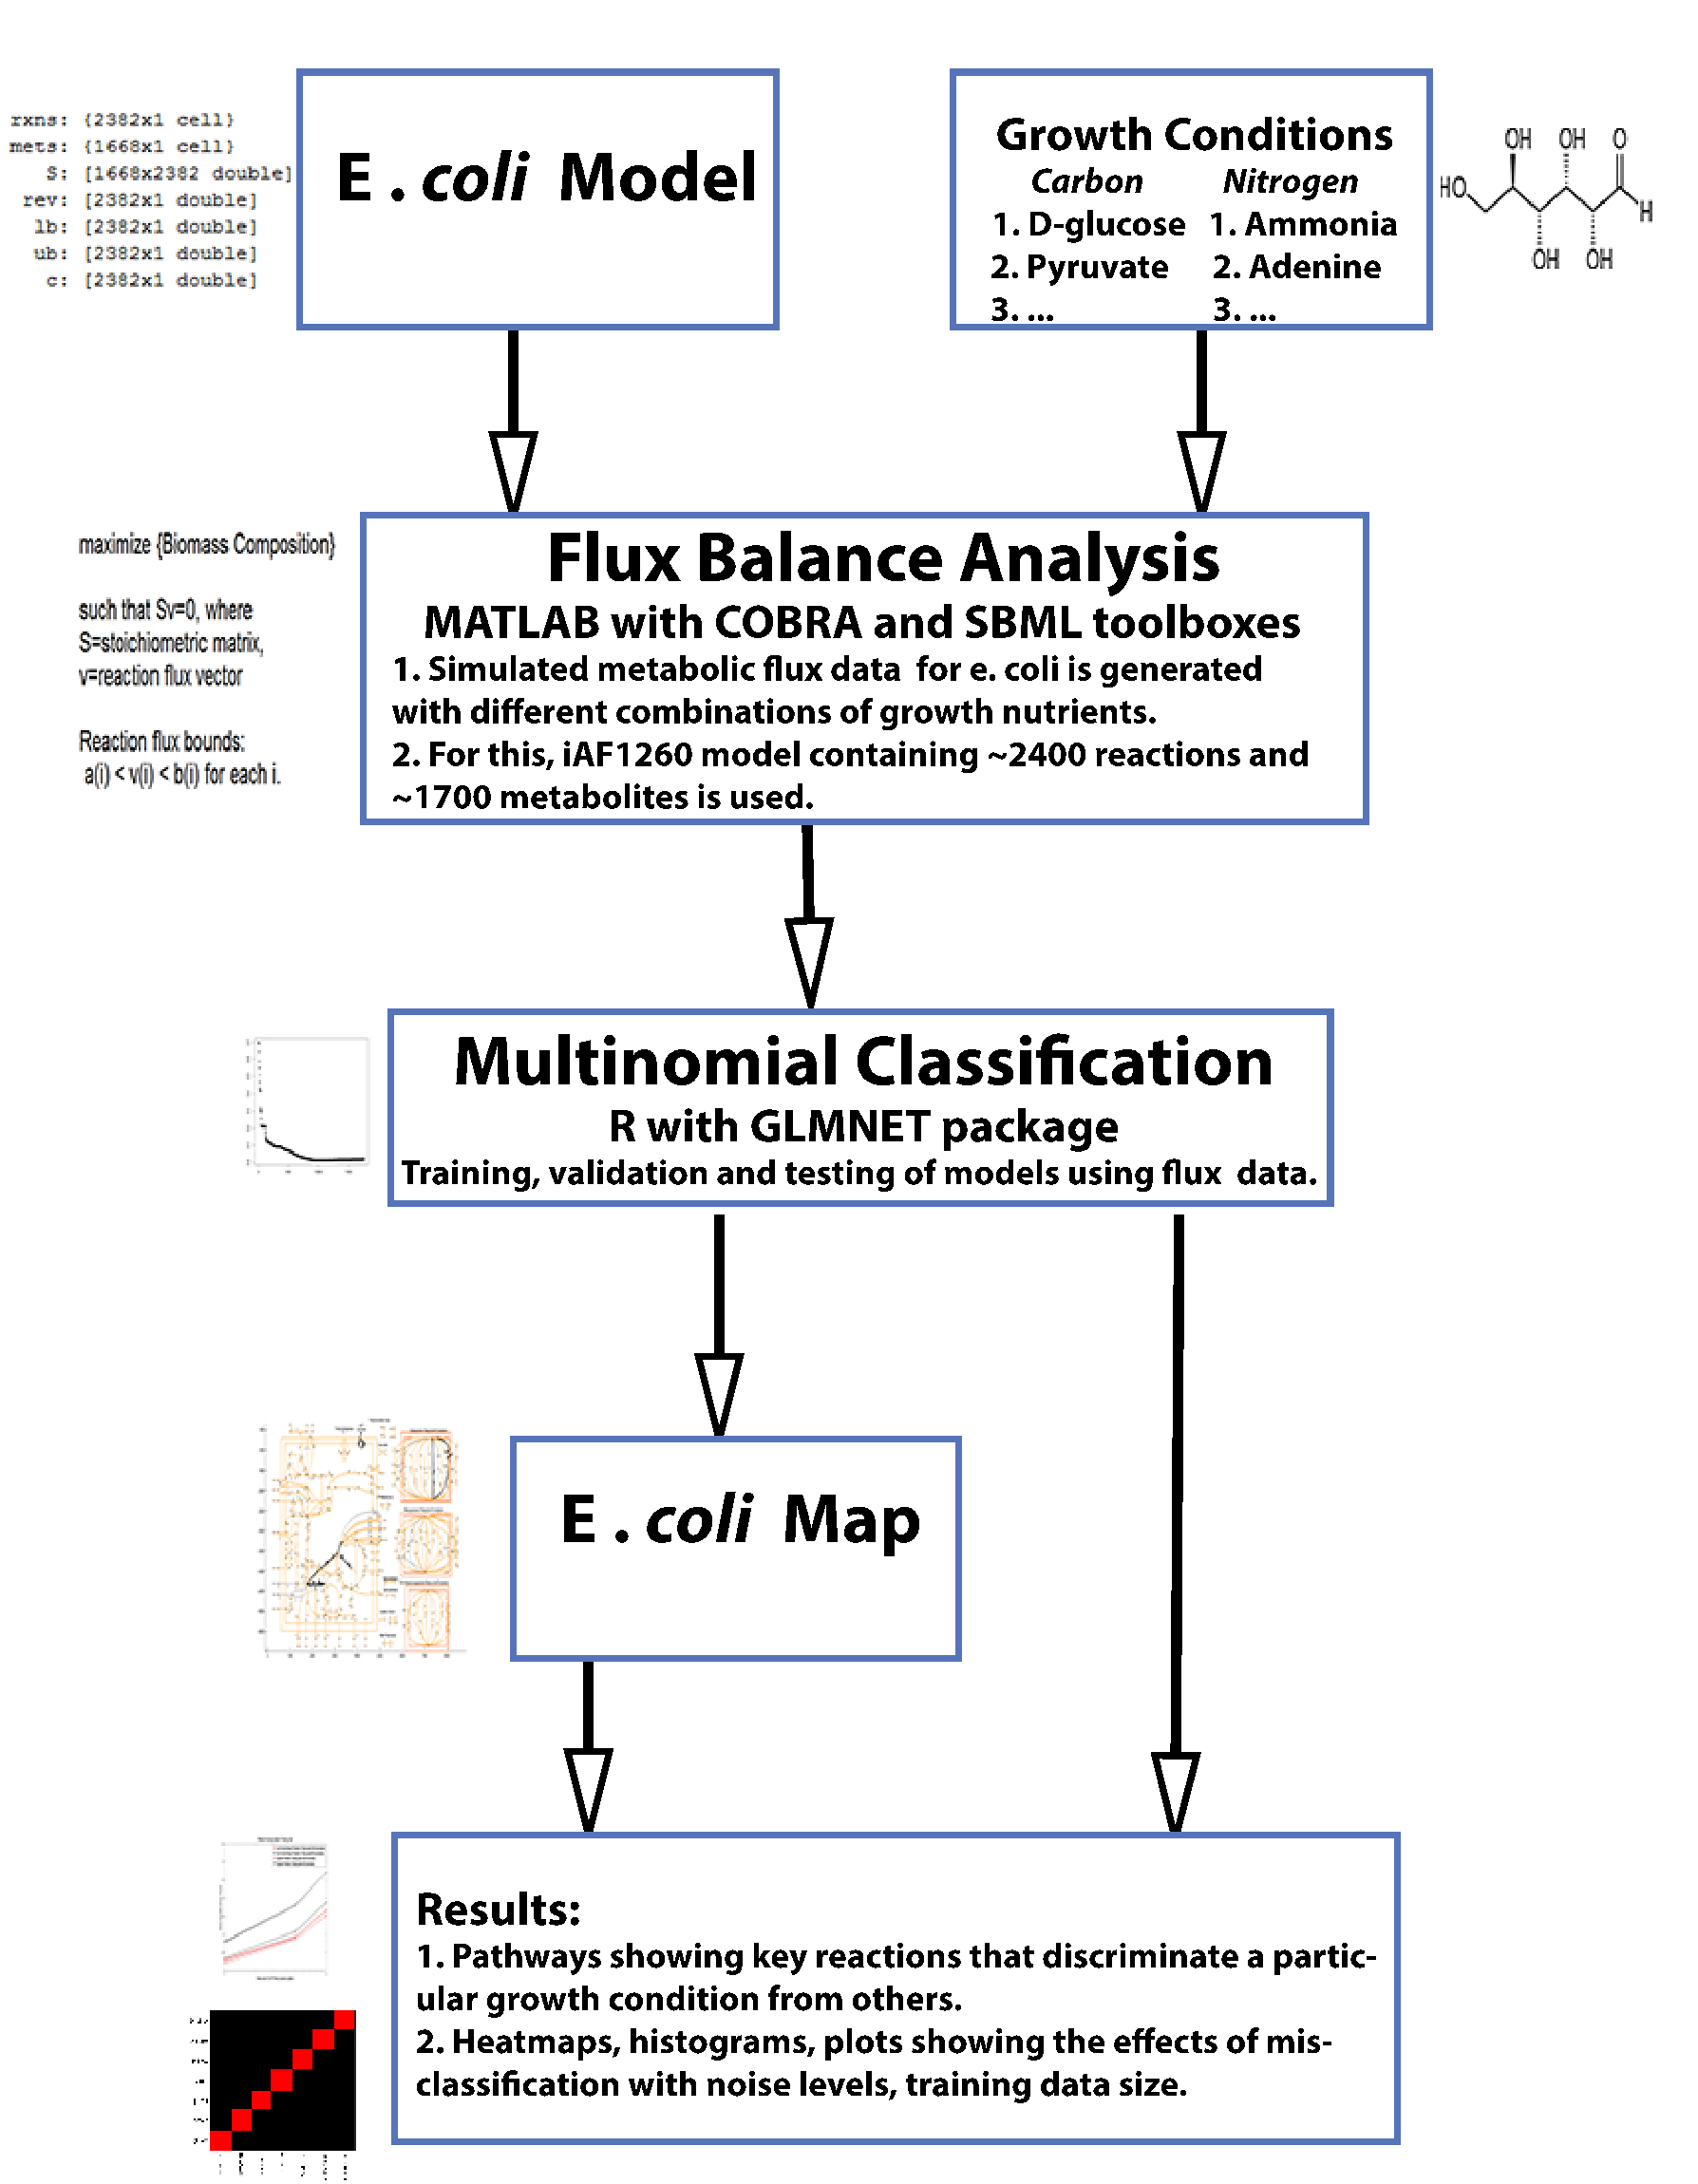
\includegraphics[width=4.5in]{Figures/flowchart_new.pdf}
\end{center}
\caption{
{\bf Flowchart describing methodology used in this study.} We obtained E. coli model and map from BiGG database. The key steps involved are Flux Balance Analysis and multinomial classification routines.
}
\label{Figure_label}
\end{figure}

\begin{figure}[!ht]
\begin{center}
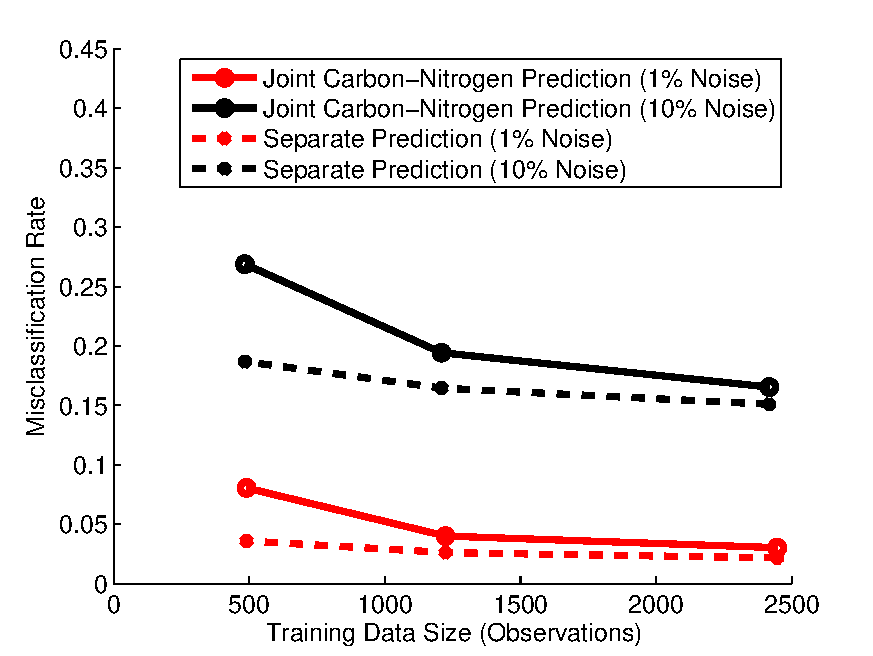
\includegraphics[width=6in]{Figures/VaryingData.pdf}
\end{center}
\caption{
{\bf Misclassification rate for different replicate sizes.} This plot shows that as training data size increases, the misclassification rate increases. This is tested for 2 different noise levels (1\% and 10\%). 
}
\label{Figure_label}
\end{figure}

\begin{figure}[!ht]
\begin{center}
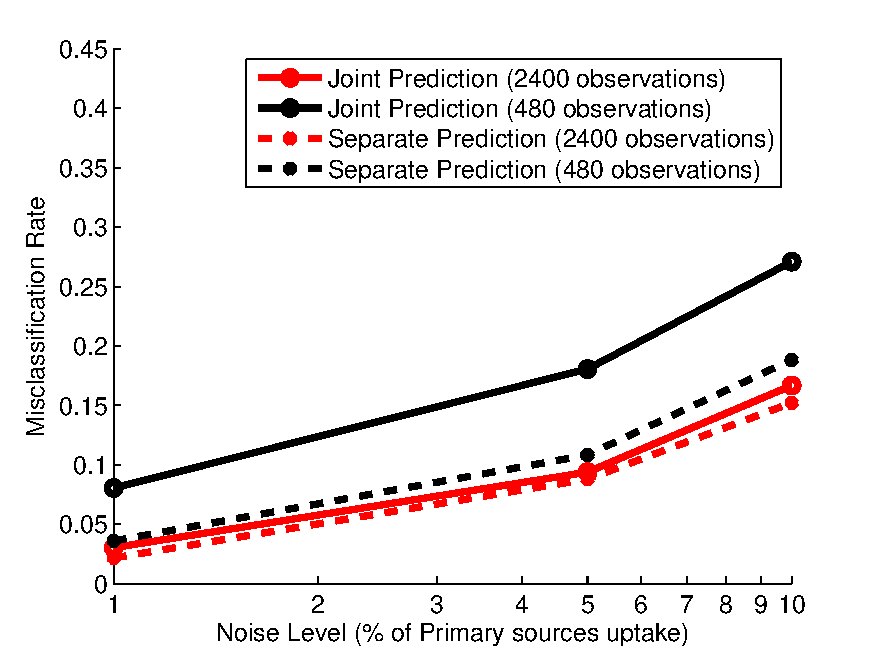
\includegraphics[width=6in]{Figures/VaryingNoise.pdf}
\end{center}
\caption{
{\bf Misclassification rate at different noise levels.} This plot shows that misclassification rate increases as noise increases in FBA models. This is tested for 2 different replicate sizes (480 and 2400 observations). 
}
\label{Figure_label}
\end{figure}

\begin{figure}[!ht]
\begin{center}
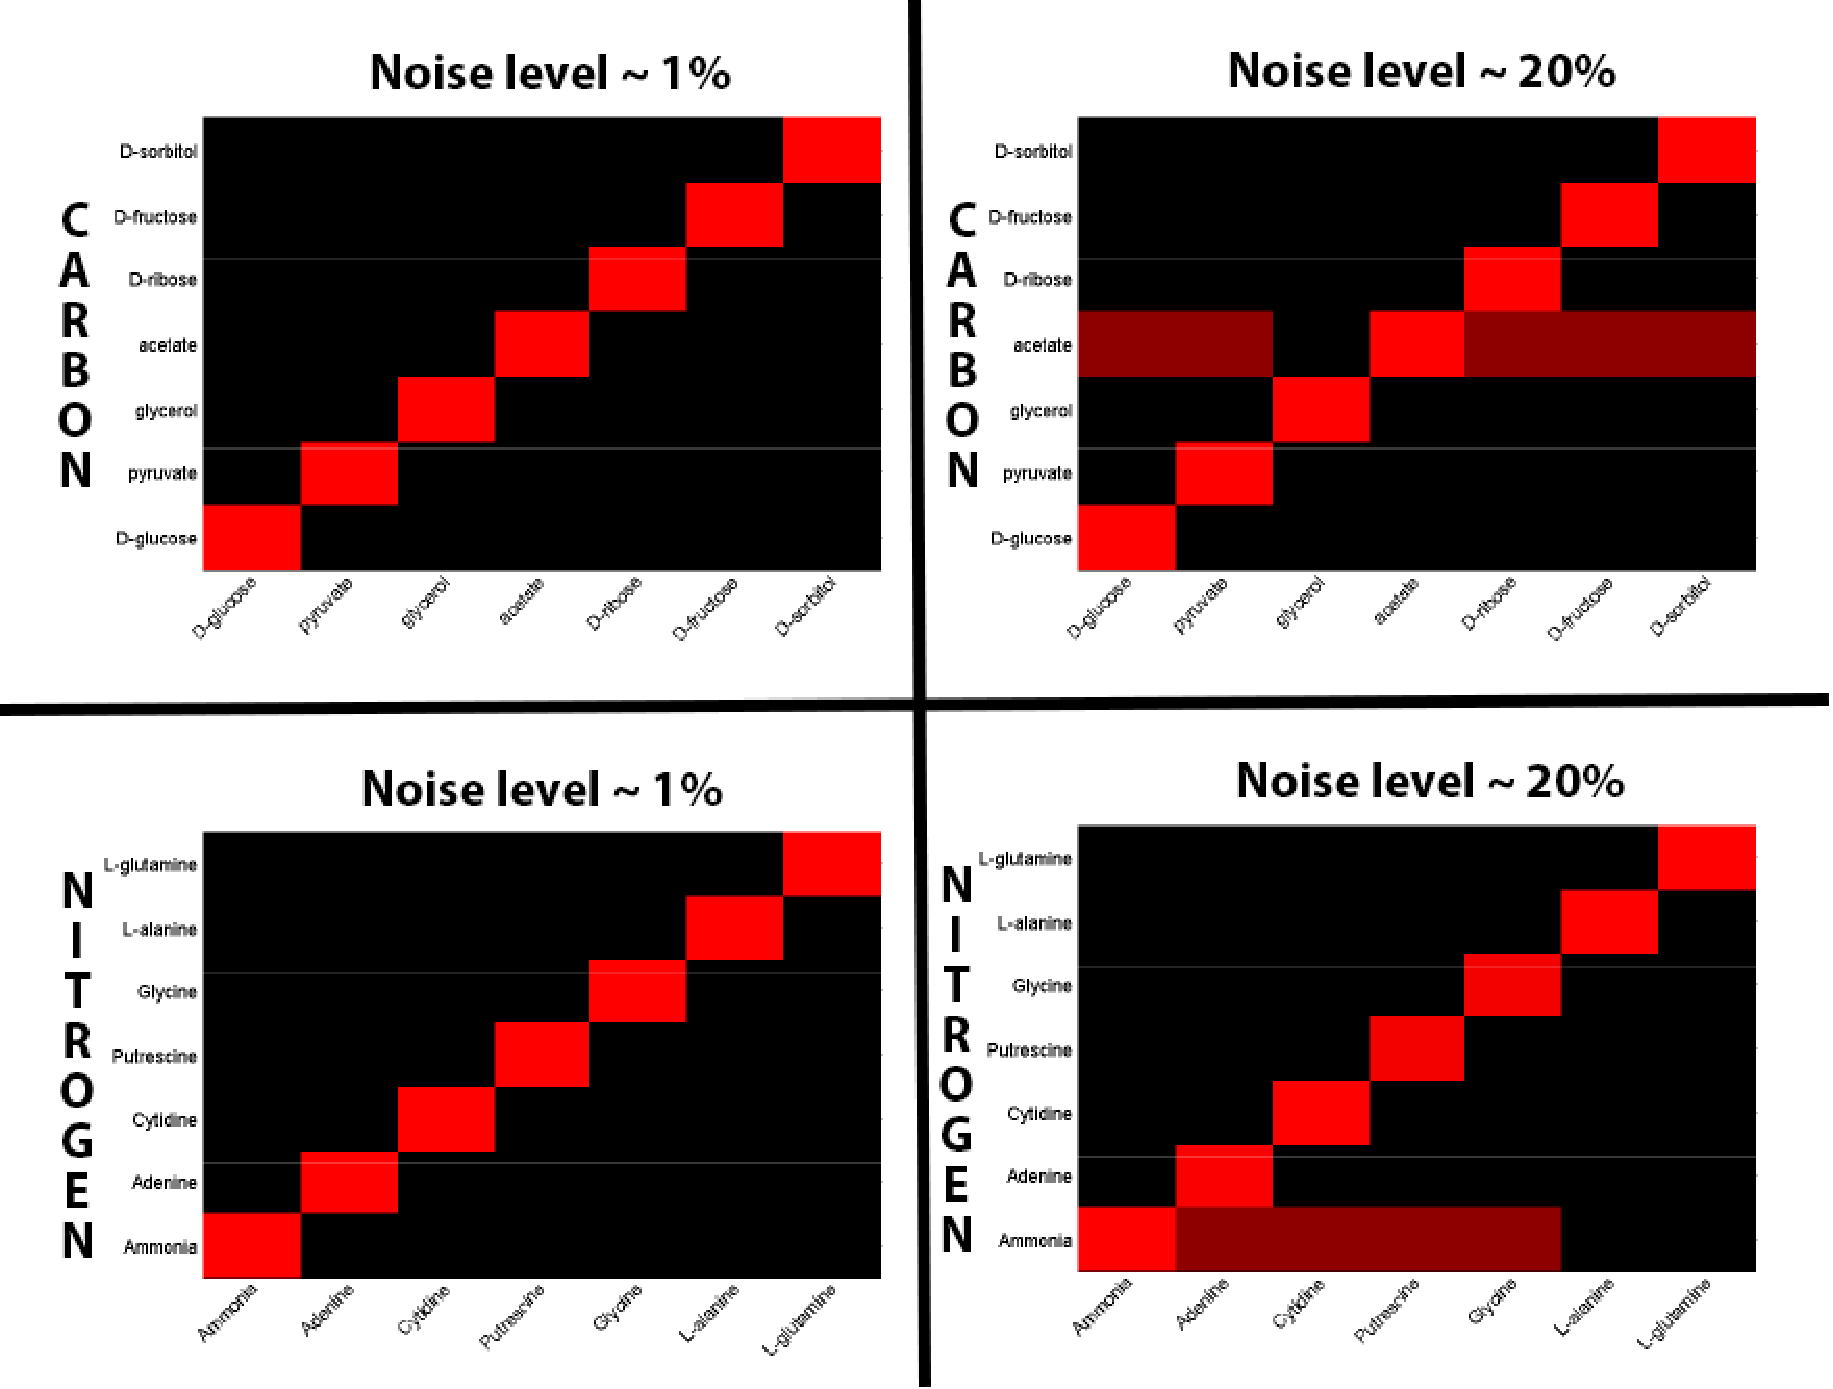
\includegraphics[width=6in]{Figures/heatmap.pdf}
\end{center}
\caption{
{\bf Heat maps with actual sources as columns and predicted ones in rows.}  At 20\% noise, most C sources are predicted to be acetate and most N sources are predicted to be ammonia.
}
\label{Figure_label}
\end{figure}

\begin{figure}[!ht]
\begin{center}
\hspace*{-3.5cm}
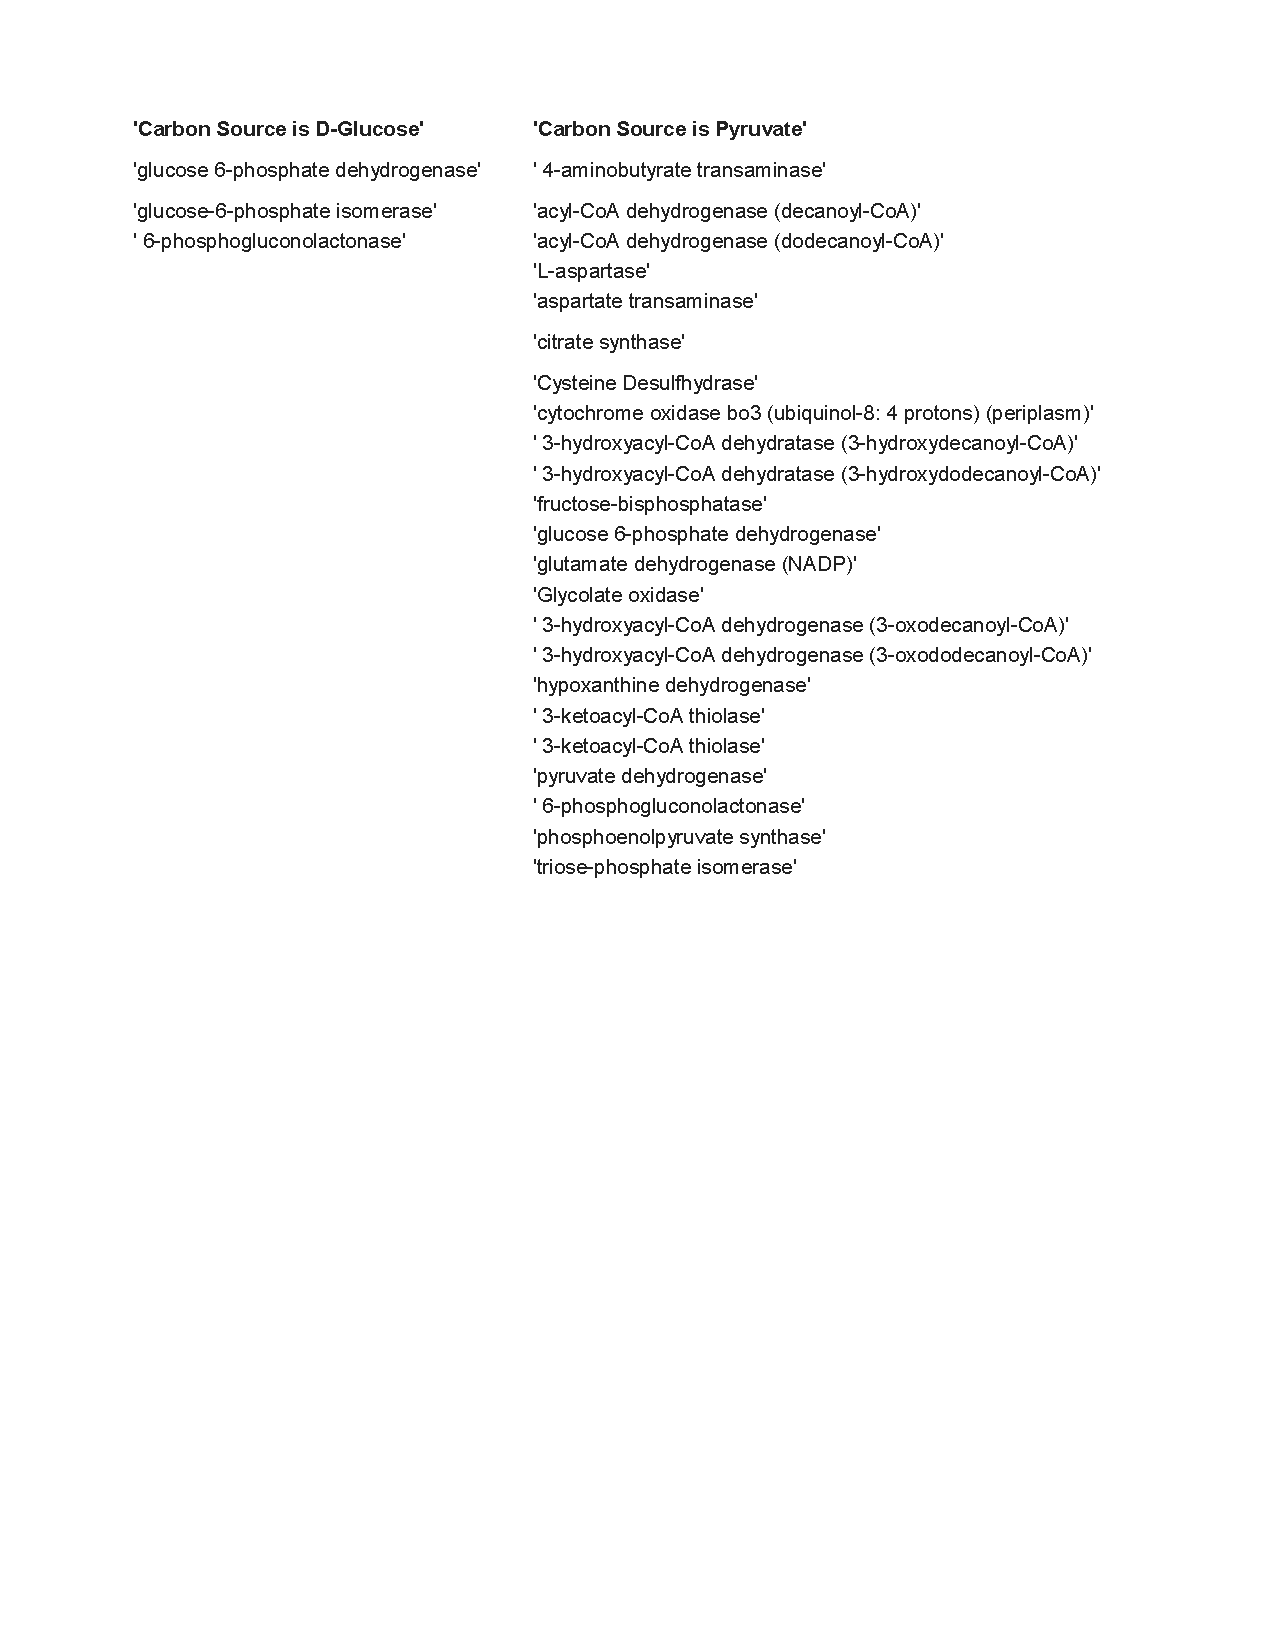
\includegraphics[width=9in]{Figures/CarbonSources.pdf}
\end{center}
\caption{
{\bf Key-reactions that discriminate Carbon sources.}  The key-reactions identified by GLMNET package were mapped onto E. coli central metabolism to visually show the differences between different growth conditions. Out of 7 carbon sources, here we show 4 carbon sources and the key-reactions.
}
\label{Figure_label}
\end{figure}

\begin{figure}[!ht]
\begin{center}
\hspace*{-3.25cm}
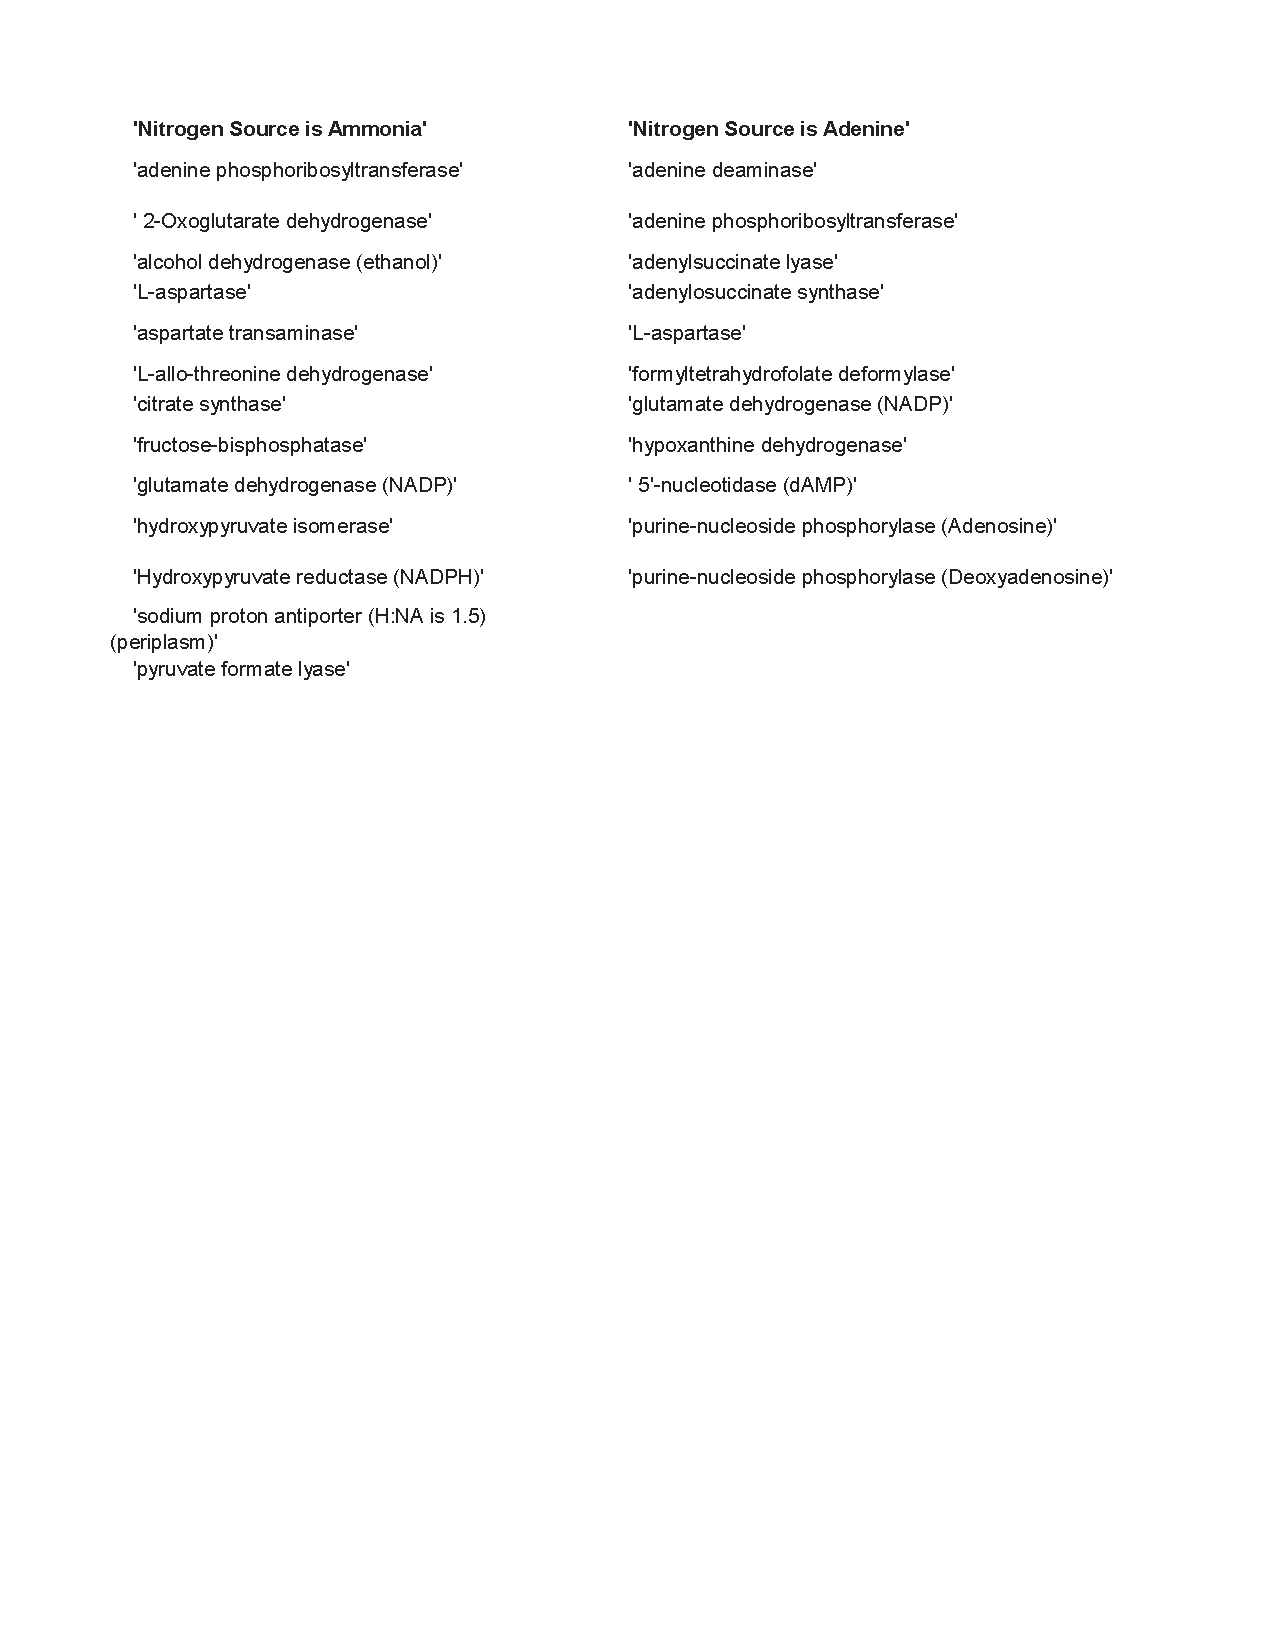
\includegraphics[width=8.5in]{Figures/NitrogenSources.pdf}
\end{center}
\caption{
{\bf Key-reactions that discriminate Nitrogen sources.}  The key-reactions identified by GLMNET package were mapped onto E. coli central metabolism to visually show the differences between different growth conditions. Out of 7 nitrogen sources, here we show 4 nitrogen sources and the key-reactions.
}
\label{Figure_label}
\end{figure}

\begin{figure}[!ht]
\begin{center}
\hspace*{-3.5cm}
\includegraphics[width=9in]{Figures/MediaSources.pdf}
\end{center}
\caption{
{\bf Key-reactions that discriminate other media.}  The key-reactions identified by GLMNET package were mapped onto E. coli central metabolism to visually show the differences between different growth conditions. Here, the growth medium used are generally used for K-12 MG1655 strain.
}
\label{Figure_label}
\end{figure}

\end{document}
